\chapter{RESEARCH METHODOLOGY}
\label{chapter_research_methodology}
This chapter describes the theoretical concept behind the methods used in this research. Architecture of the proposed handwriting recognition system is given in chapter \ref{chapter_system_overview}. Subsections of this chapter are organized as follows.\par
Section \ref{section_preprocessing_methodology} describes the image preprocessing techniques. Feature extraction techniques are described in the section \ref{section_feature_extraction_methodology}. System training and testing methods are described in the section \ref{section_training_testing_methodology}.

\section{Image Preprocessing}\label{section_preprocessing_methodology}

Image preprocessing is the preliminary step of the recognition procedure. Preprocessing describes how images are normalized before extracting features from it. Region of interest is selected from given character image and make it fine conditioned. This section provides the detail description about steps used in preprocessing of given character images. The main steps of image preprocessing are given in algorithm \ref{algorithm_preprocessing}.

\begin{algorithm}
\caption{Image Preprocessing}
\label{algorithm_preprocessing}
\begin{algorithmic}[1]
\STATE  Read image.
\STATE  Convert RGB images to gray scale image.
\STATE  Remove noise using median filter.
\STATE  Convert the gray scale images to binary image.
\STATE	Image Inversion (making background black \& foreground white).
\STATE  Determine the universe of discourse of image.
\STATE  Normalize the image to a predefined size of 36x36 pixels.
\STATE  Convert the normalized image to single pixel thick skeleton image.
\end{algorithmic}
\end{algorithm}

Following subsections describe each of these steps in detail. The organization of subsections are as follows: Color normalization method is described in section \ref{section_rgb_to_gray_conversion}, noise removal is described in section \ref{section_noise_removal}, image segmentation procedure is described in the section \ref{section_image_segmentation}, image inversion is given in section \ref{section_image_inversion}, universe of discourse selection technique is presented in the section \ref{section_discourse}, size normalization method is given in section \ref{section_size_normalization} and image skeletonization process is described in the section \ref{section_skeletonization}.

%Character slant and skew correction are two another important steps of image preprocessing.But in this research work slant and skew correction is no more needed since images are itself in fine  condition.


\subsection{RGB to Grayscale Conversion}\label{section_rgb_to_gray_conversion}

Given $24$ bit true colour RGB image is converted into $8$ bit grayscale image. Grayscale component is calculated by taking weighted summation of R, G and B components of RGB image. Weights are selected same as the NTSC color space selects for the luminance i.e. the grayscale signal used to display pictures on monochrome televisions. For the RGB image $f(x,y)$, corresponding graysclae image is given by,
\begin{equation}
g(x,y)= 0.2989 * R(f(x,y)) + 0.5870 *G(f(x,y)) + 0.1140 * B(f(x,y))
\end{equation}

where, $R(f(x,y))$ is red component of the RGB image $f(x,y)$, and so on.

Figure \ref{figure_grayed} shows the RGB to grayscale conversion of input image.
\begin{figure}[h]
\centering
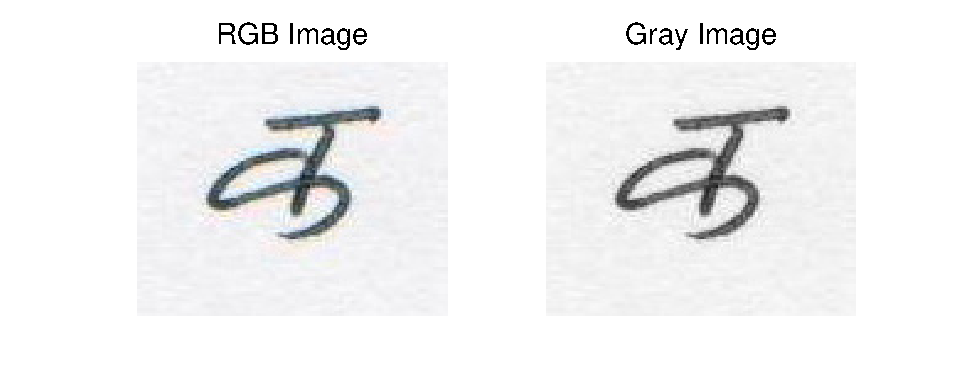
\includegraphics[width=4in]{figures/ka_preprocessing/grayed.eps}
\caption{RGB to Grayscale Conversion.}
\label{figure_grayed}
\end{figure}


\subsection{Noise Removal}\label{section_noise_removal}

Noise removal is one of the important step of image preprocessing. Any unnecessary pixels are removed with the help of filtering. Non-linear median filtering technique is used for noise removal. Median filter is an effective method of noise removal which can suppress isolated noise without blurring sharp edges. Median filter replaces a pixel with the median value of its neighbourhood. For the digital image $f(x,y)$, median filtered image is obtained as,
\begin{equation}
g(x,y)= median\{f(i,j)\;\vline \;(i,j)\in \; w \}
\end{equation}
where, $w$ is the neighbourhood centered around location $(x,y)$ in the image.
Figure \ref{figure_denoised} shows the denoised image corresponding to given grayscaled image.
\begin{figure}[hbtp]
\centering
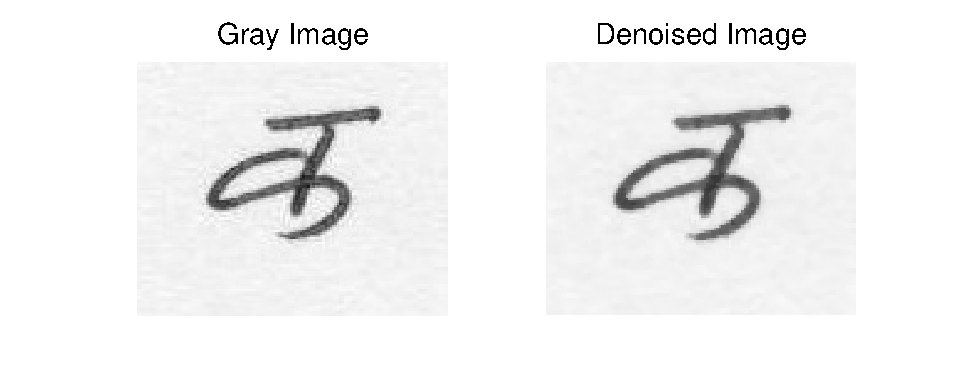
\includegraphics[width=4in]{figures/ka_preprocessing/denoised.eps}
\caption{Noise Removal.}
\label{figure_denoised}
\end{figure}
\subsection{Image Segmentation}\label{section_image_segmentation}

Segmentation is the central problem of distinguishing object from the background. There are many algorithms for image segmentation. This section describes the thresholding method with Otsu's threshold selection technique \cite{Otsu1979} for grayscale image segmentation.

Otsu's graylevel threshold selection method for image binarization is a nonparametric and unsupervised method of automatic threshold selection. An optimal threshold is selected by the discriminant criteria i.e., by maximizing the interclass variance between white and black pixels. Image segmentation algorithm for grayscale image is given in Algorithm \ref{algorithm_segmentation}. Figure \ref{figure_binarized} shows binarized image of given grayscale image.
\begin{figure}[h]
\centering
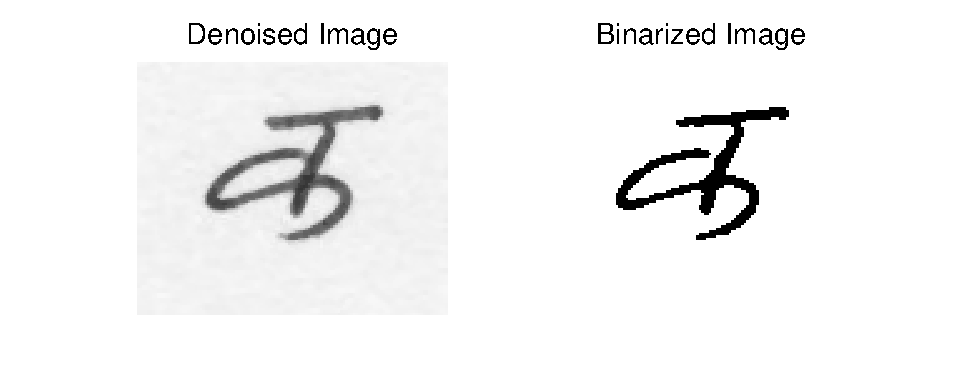
\includegraphics[width=4in]{figures/ka_preprocessing/binarized.eps}
\caption{Image Binarization.}
\label{figure_binarized}
\end{figure}

\begin{algorithm}
\caption{Image Binarization}
\label{algorithm_segmentation}
\begin{algorithmic}[1]
\STATE  Compute histogram and probability of each intensity level $i$ , $i=1\cdots L$.
\STATE  Compute between class variance for black and white pixels, by taking threshold $ t=1\cdots L$, \par
\STATE \qquad $\sigma^2_b(t)=\omega_1(t)\omega_2(t)[\mu_1(t)-\mu_2(t)]^2$ \par
\qquad\qquad where,\par
\STATE \qquad\qquad\qquad $\omega_1(t)=\sum\limits_{1}^{t} p(i) $ is the class probability for black pixels,\par
\STATE \qquad\qquad\qquad $\omega_2(t)=\sum\limits_{t+1}^{L} p(i) $ is the class probability for white pixels,\par

\STATE \qquad\qquad\qquad $\mu_1(t)=\sum\limits_{1}^{t} \frac{ip(i)}{\omega_1(t)}$ is the class mean for black pixels,\par
\STATE \qquad\qquad\qquad $\mu_2(t)=\sum\limits_{t+1}^{L} \frac{ip(i)}{\omega_2(t)}$ is the class mean for white pixels,\par
\STATE \qquad\qquad\qquad and, $p(i)$ is the probability of intensity level $i$.

\STATE Select $t$ for which $\sigma^2_b(t)$ is maximum.
\STATE Finally, binarize the grayscale image $f(x,y)$ using the threshold $t$ as,\par
\STATE \qquad $g(x,y)=\left\{
\begin{array}{c l}
    1 & if \; f(x,y)\ge t\\
    0 & if \; f(x,y)\; \textless\;t
\end{array}\right.$


\end{algorithmic}
\end{algorithm}


\subsection{Image Inversion}\label{section_image_inversion}

Handwritten documents are normally written in white paper with black pen. For the recognition system, we assume black pixels as a background and white pixels as the foreground. So, captured images are inverted before passing into the recognition engine. The inverted image of binary image $f(x,y)$ can be obtained by the negative transformation as,
\begin{equation}
g(x,y)=1-f(x,y)
\end{equation}
Figure \ref{figure_inverted} shows the negative image of given binary image.
\begin{figure}[h]
\centering
\includegraphics[width=4in]{figures/ka_preprocessing/inverted.eps}
\caption{Image Negatives.}
\label{figure_inverted}
\end{figure}

\subsection{Universe of Discourse}\label{section_discourse}
Determining universe of discourse of the character image is finding smallest rectangle that encloses the character object. It removes extra pixels outside the convex hull of the character image. Figure \ref{figure_discoursed} shows the discoursed image of given binary image.
\begin{figure}[h]
\centering
\includegraphics[width=4in]{figures/ka_preprocessing/discoursed.eps}
\caption{Universe of Discourse.}
\label{figure_discoursed}
\end{figure}

\subsection{Size Normalization}\label{section_size_normalization}
Size normalization is the technique of converting all the variable size input images to fixed size images. Size normalization is done so that we do not require paddings of pixels at the time of feature extraction. All the input images are normalized to the predefined size of $36$x$36$ pixels. Figure \ref{figure_size_normalized} shows the size normalized image.
\begin{figure}[h]
\centering
\includegraphics[width=4in]{figures/ka_preprocessing/size_normalized.eps}
\caption{Size Normalization.}
\label{figure_size_normalized}
\end{figure}

\subsection{Image Skeletonization}\label{section_skeletonization}
Skeletonization is a process for reducing object regions in a binary image to a skeletal remainder that largely preserves the extent and connectivity of the original object while throwing away most of the original object pixels. It plays an important role in the preprocessing phase of handwriting recognition. Skeletonization creates single pixel wide connected object boundary, that preserves euler number of the original object. There are many reasons behind skeletonization of the binary image such as, to reduce the amount of data and time for processing the image, to extract critical features like end-points, intersection-points, connections etc., to help in shape analysis algorithms, and so on. Skeletonization calculates a medial axis skeleton so that points of this skeleton are at the same distance of its nearby borders. Image thinning algorithm is first given by Harry Blum (1967) \cite{Blum1967}. Binary image skeletonization is carried out by the object thinning procedure that iteratively delete boundary points of a region object to the constraints that deletion of these points; (1) does not remove end points, (2) does not break connectivity and (3) does not cause excessive erosion of the region. \ac{mat} algorithm \cite{Gonzalez2008} for  binary image thinning  is given in algorithm \ref{algorithm_skeletonization}. The MAT of a object region has an intuitive definition based on the so-called ``prairie fire concept''. Consider an image region, as a prairie of uniform dry grass, and suppose a fire it lit along its border. All fire fronts will advance into the region at the unique speed. The \ac{mat} of the object region is then the set of points reached by more than one fire front at the same time. Figure \ref{figure_skeletonized} shows the skeletonized image of given binary image.

\begin{algorithm}
\caption{Image Skeletonization Algorithm}
\label{algorithm_skeletonization}
\begin{algorithmic}[1]
\STATE Repeat following steps until no contour points.
\STATE \qquad (a) Delete all contour points according to Definition 1.
\STATE \qquad (b) Delete all contour points according to Definition 2.
\STATE Definition 1: For contour point $P1$ (see table right for the 8- connected relationship) that satisfies following conditions,

\begin{tabular}{cc}
\qquad
\begin{tabular}{ll}
(a) 2 $\le$ $N(P1)$ $\le$ 6 &  \\
(b) $T(P1)=1$ &  \\
(c) $P2.P4.P6=0$ &  \\
(d) $P4.P6.P8=0$ &  \\
\end{tabular}
&
$\begin{tabular}[r]{|c|c|c|r}
\hline P9 & P2 & P3 \\
\hline P8 & P1 & P4 \\
\hline P7 & P6 & P5 \\
\hline
\end{tabular} $
\end{tabular}
\tablename{: The 8- connected relationship}

where $N(P1)$ is the number of non-zero neighbours of $P1$: $N(P1)= \sum\limits_{i=2}^{9} P_i$, and $T(P1)$ is the number of 0-1 transitions in the ordered sequence $P2,P3,\cdots,P9,P2$ (clockwise).
\STATE Definition 2: For contour point $P1$ that satisfies the following conditions

\qquad
\begin{tabular}{ll}
(a) same as above & \\
(b) same as above &  \\
(c$^\prime$) $P2.P4.P8=0$ &  \\
(d$^\prime$) $P2.P6.P8=0$ &  \\
\end{tabular}
\end{algorithmic}
\end{algorithm}

%Description of image skeletonization algorithm \ref{algorithm_skeletonization} can be given as, condition (a) shows if there is only one 1 in the neighborhood, $P1$ is an end point and should not be deleted; if there are seven 1’s, deleting p1 would cause erosion; if there are eight 1’s, $P1$ is not a contour point, condition (b) shows $P1$ is an arc point and deleting $P1$ would break the connectivity, conditions (c) and (d) shows right, bottom, and upper left corner contour points, ans condition (c$^\prime$) and (d$^\prime$) shows the top, left and lower right corner contour points.

\begin{figure}[h]
\centering
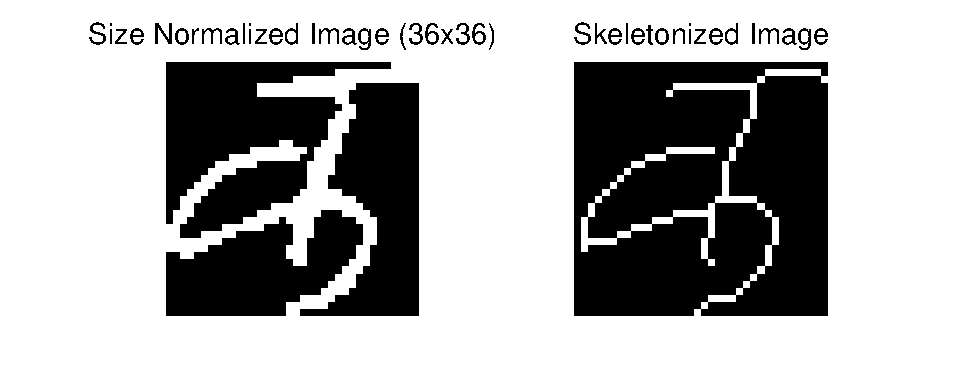
\includegraphics[width=4in]{figures/ka_preprocessing/skeletonized.eps}
\caption{Binary Image Skeletonization.}
\label{figure_skeletonized}
\end{figure}

\newpage
\section{Feature Extraction}\label{section_feature_extraction_methodology}
After Pre-processing of the character images the next stage of character recognition is feature extraction. Feature extraction step plays one of the most important roles in the recognition. It is the heart of recognition system. A good feature set should represent  characteristic of the class that helps distinguish it from other classes, while remaining invariant to characteristic differences within the class. Hundreds of features are available in the literature \cite{Jain1996,Jain2000,Zhang2004}.

This section describes features extraction techniques. Combination of statistical features (Moment Invariants, Centroid and Area) and geometric features ( Directional Features, Euler Number and Eccentricity) are used to describe the character property. These features are extracted from individual preprocessed handwritten character images.

\subsection{Directional Features}
\label{section_directional_features}
Directional features are extracted from skeletonized character image based on the basic line types that form the skeleton of the character. These topological features may represent global and local properties of the object along with some knowledge about the contour of the object or some knowledge about the components of the object.
This technique implements the idea given in \cite{Blumenstein2003}. Each pixel in the image is traversed. Individual line segments, there directions and intersection points are identified from segmented character image.

For this, given pre-processed character image is zoned into 3x3 windows of equal size. Then number, length, type of lines and intersection points are identified in each zone. The line segment that would be determined in each zone is categorized into four types: vertical lines, horizontal lines, right diagonal lines and left diagonal lines. To extract direction features, the following steps are required,

\begin{enumerate}
\itemsep0em
\item Starting points and intersection point identification.
\item Individual line segment identification.
\item Labelling line segment.
\item Line type normalization.
\end{enumerate}

From each zone of the character image following properties are extracted \cite{Gaurav2012}.
\begin{enumerate}
\itemsep0em
\item Number of horizontal lines.
\item Number of vertical lines.
\item Number of Right diagonal lines.
\item Number of Left diagonal lines.
\item Normalized Length of all horizontal lines.
\item Normalized Length of all vertical lines.
\item Normalized Length of all right diagonal lines.
\item Normalized Length of all left diagonal lines.
\item Number of intersection points.
\end{enumerate}
It results feature vector of dimensional 9 for each zone. A total of 81 (9x9) features are obtained.

\subsection{Moment Invariant Features}
\label{section_moment_invariant_features}
Moment invariants are important tools in object recognition problem. These techniques grab the property of image intensity function. Moment invariants were first introduced to the pattern recognition community in 1962 by Hu \cite{Hu1962}, who employed the results of the theory of algebraic invariants and derived his seven famous invariants to rotation of 2-D objects. Moment invariants used in this research for extracting statistical patterns of character images are given in \cite{Gonzalez2008}. Moment invariants are pure statistical measures of the pixel distribution around the centre of gravity of the character and allow capturing the global character shape information.

The standard moments $m_{pq}$ of order $(p+q)$ of an image intensity function $f(x,y)$ is given by,

\begin{equation}\label{equation_moments}
m_{pq}=\int\limits_{-\infty}^{\infty}\int\limits_{-\infty}^{\infty}x^py^qf(x,y)dxdy \;\;  p,q = 0,1 , 2, ...
\end{equation}
A uniqueness theorem states that if $f(x,y)$ is piecewise continues and has non-zero values only in a finite part of the $x_{vis},y_{vis}$ plane, moments of all order exist and the moment sequence $(m_{pq})$ is uniquely determined by $f(x,y)$. Conversely, $(m_{pq})$ is uniquely determines $f(x,y)$.

%For discrete domain, Eq.(\ref{equation_moments}) is transformed by summing over sub-image within which object of interest lies, to get the standard moments of order $(p+q)$.
For discrete domain, the 2-D moment of order $(p+q)$ for a digital image $f(x,y)$ of size $M$x$N$ is given by,

\begin{equation}\label{equation_digital_moments}
m_{pq}=\sum\limits_{x=0}^{M-1}\sum\limits_{y=0}^{N-1}x^py^qf(x,y) \;\;  p,q = 0,1 , 2, ...
\end{equation}
The corresponding central moment of order $(p+q)$ is defined as,
\begin{equation}\label{equation_central_digital_moments}
\mu_{pq}=\sum\limits_{x=0}^{M-1}\sum\limits_{y=0}^{N-1}(x-\bar{x})^p(y-\bar{y})^qf(x,y) \;\;  p,q = 0,1 , 2, ...
\end{equation}
where,
\begin{equation}\label{equation_xbar_ybar}
\bar{x}=\frac{m_{10}}{m_{00}} \; and \; \bar{y}=\frac{m_{01}}{m_{00}}
\end{equation}
The normalized central moments, denoted by $\eta_{pq}$, are defined as,
\begin{equation}\label{equation_central_normalized_moments}
\eta_{pq}=\frac{\mu_{pq}}{\mu^{\gamma}_{00}}
\end{equation}
where,
\begin{equation}\label{equation_gamma}
\gamma=\frac{p+q}{2}+1 \;\; for\;\; p+q=2,3,...
\end{equation}
A set of seven invariant moments can be derived from the second  and third moments \cite{Hu1962} which are invariant to translation, scale change, mirroring, and rotation, are given as follows.

\begin{subequations}
\begin{align}
\phi_1 &=\eta_{20}+\eta_{02} \\
\phi_2&=(\eta_{20}-\eta_{02})^2+4\eta^2_{11} \\
\phi_3&=(\eta_{30}-3\eta_{12})^2+(3\eta_{12}-\eta_{03})^2 \\
\phi_4&= (\eta_{30}+\eta_{12})^2+(\eta_{21}+\eta_{03})^2 \\
%\begin{split}
\phi_5&=(\eta_{30}-3\eta_{12})(\eta_{30}+\eta_{12})[(\eta_{30}-3\eta_{12})^2-3(\eta_{12}+\eta_{03})^2] \nonumber \\
&\qquad +(3\eta_{21}-\eta_{03})(\eta_{21}+\eta_{03})[3(\eta_{30}+\eta_{12})^2-(\eta_{21}+\eta_{03})^2] \\
\phi_6&=(\eta_{20}-\eta_{02})[(\eta_{30}+\eta_{12})^2-(\eta_{21}+\eta_{03})^2] \nonumber \\
&\qquad +4\eta_{11}(\eta_{30}+\eta_{12})(\eta_{21}+\eta_{03}) \\
\phi_7&=3(\eta_{21}-\eta_{03})(\eta_{30}+\eta_{12})[(\eta_{30}+\eta_{12})^2-3(\eta_{21}+\eta_{03})^2] \nonumber\\
&\qquad +3(\eta_{12}-\eta_{30})(\eta_{21}+\eta_{03})[3(\eta_{30}+\eta_{12})^2-(\eta_{21}+\eta_{03})^2]
%\end{split}
\end{align}
\end{subequations}


\subsection{Euler Number}
\label{section_euler_number}
Euler number is the difference of number of objects and the number of holes in the image. This property is affine transformation invariant. Euler number is computed by considering patterns of convexity and concavity in local 2-by-2 neighbourhoods \cite{Pratt1991}. Euler number can be calculated by using local information and does not require connectivity information. Calculating the Euler number of a binary image can be done by counting the occurrences of three types of 2x2 binary patterns.

%P1=(1 0  0 1  0 0  0 0)
%    0 0, 0 0, 1 0, 0 1
%P2=(0 1  1 0  1 1  1 1)
%    1 1, 1 1, 0 1, 1 0
%P3=(1 0  0 1)
%    0 1, 1 0
%
$$ P1=
\left(
  \begin{array}{ccccccccccc}
    1 & 0 &  & 0 & 1 &  & 0 & 0 &  & 0 & 0 \\
    0 & 0 &, & 0 & 0 &, & 0 & 1 &, & 1 & 0 \\
  \end{array}
\right)
$$

$$ P2=
\left(
\begin{array}{ccccccccccc}
    0 & 1 &  & 1 & 0 &  & 1 & 1 &  & 1 & 1 \\
    1 & 1 &, & 1 & 1 &, & 1 & 0 &, & 0 & 1 \\
\end{array}
\right)
$$
$$ P3=
\left(
\begin{array}{ccccc}
1&0& &0&1 \\
0&1&,&1&0 \\
\end{array}
\right)
$$

Let $C1$, $C2$ and $C3$ be the number of occurrences of patterns $P1$, $P2$ and $P3$ respectively, then the Euler Number for the image with 4- and 8-connectivity is simply given as \cite{Pratt1991},

\begin{equation}
E_4=\frac{1}{4}(C1-C2+2C3)
\end{equation}
\begin{equation}
E_8=\frac{1}{4}(C1-C2-2C3)
\end{equation}
%Reference: Pratt, William K., Digital Image Processing, New York, John Wiley and Sons, Inc., 1991, p. 633.

\subsection{Normalized Area of Character Skeleton}
\label{section_area}
The area of the object within the binary image is simply the count of the number of pixels in the object for which $ f(x,y)=1 $. Normalized regional area is the ratio of the number of the pixels in the skeleton of binary image to the total number of pixel in the image.

\subsection{Centroid of Image}
\label{section_centroid}

Centroid specifies the center of mass of the object region in given image. Horizontal centroid coordinate is calculated by dividing the sum of all horizontal positions of the object which are non zero with area of the object. Similarly, vertical centroid coordinate is calculated by dividing the sum of all vertical positions of the object which are non zero with area of the object. Centroid coordinates of the binary image $f(x,y)$ of size $M$x$N$ are given in equation \ref{equation_centroidx_centroidy},

\begin{subequations}\label{equation_centroidx_centroidy}
\begin{align}
centroid_x=\frac{m_{10}}{m_{00}} = \dfrac{\dfrac{1}{N}\sum\limits_{i=0}^{M-1}\sum\limits_{j=0}^{N-1}x_jf(i,j)}{\sum\limits_{i=0}^{M-1}\sum\limits_{j=0}^{N-1}f(i,j)}\\\nonumber\\
centroid_y=\frac{m_{01}}{m_{00}} = \dfrac{\dfrac{1}{M}\sum\limits_{i=0}^{M-1}\sum\limits_{j=0}^{N-1}y_jf(i,j)}{\sum\limits_{i=0}^{M-1}\sum\limits_{j=0}^{N-1}f(i,j)}
\end{align}
\end{subequations}


\subsection{Eccentricity}
\label{section_eccentricity}
The eccentricity is the ratio of the distance between the foci of the ellipse that best fit the character object and its major axis length. Eccentricity describes the rectangularity of the region of the object. The measure of eccentricity can be obtained by using the minor and major axes of such an ellipse \cite{Rosin1999}. This method of calculating eccentricity uses the second order moments. The eccentricity of the ellipse is given by,

%\begin{equation}
%e=\frac{(\mu_{20}-\mu_{02})^2+4(\mu_{11})^2}{\mu_{00}}
%\end{equation}

\begin{equation}
e=\sqrt{\dfrac{\alpha^2-\beta^2}{\alpha^2}}
\end{equation}

where $\alpha$ and $\beta$ are semi-major axis and semi-minor axis of the ellipse respectively, which are given by,

\begin{equation}
\alpha=\sqrt{\dfrac{2[\mu_{20}+\mu_{02}+\sqrt{(\mu_{20}-\mu_{02})^2+4\mu_{11}^2}]}{\mu_{00}}}
\end{equation}

\begin{equation}
\beta=\sqrt{\dfrac{2[\mu_{20}+\mu_{02}-\sqrt{(\mu_{20}-\mu_{02})^2+4\mu_{11}^2}]}{\mu_{00}}}
\end{equation}

where $\mu_{pq}$ is as described in equation \ref{equation_central_digital_moments}.

%The eccentricity of a circle is zero. The eccentricity of an ellipse which is not a circle is greater than zero but less than 1. This is a measure of how a circular object deviates deviates from circularity. A perfectly circular body has an eccentricity of zero. Higher values of eccentricity is an indication of more elliptical shape.

\section{Training and Testing}\label{section_training_testing_methodology}

After the feature extraction phase, process of training and testing begins. In the training phase, recognition system learns patterns of different classes from input feature vectors. The learning is done in supervised manner. After the training phase, system is ready to test in unknown environment. Recognition system is then tested against testing feature vectors and accuracy and efficiency of the system is calculated. In this research, recognition is carried out using two neural network algorithms, multilayer feedforward neural network with \ac{lm} and \ac{gdma} learning and radial basis function networks with \ac{ols} learning. Section \ref{section_multilayer_feedforward_network} describes the \ac{mlp} algorithm and section \ref{section_radial_basis_function} describes the RBF algorithm.

\subsection{Multilayer Feedforward Backpropagation Network}
\label{section_multilayer_feedforward_network}

A multilayer feedforward neural network consists of a layer of input units, one or more layers of hidden units, and one layer of output units. A neural network that has no hidden units is called a Perceptron. However, a perceptron can only represent linear functions, so it isn't powerful enough for the kinds of applications we want to solve. On the other hand, a multilayer feedforward neural network can represent a very broad set of non-linear functions. So, it is very useful in practice. This multilayer architecture of Network determines how the input is processed. The network is called feedforward because the output from one layer of neurons feeds forward into the next layer of neurons. There are never any backward connections, and connections never skip a layer. Typically, the layers are fully connected, meaning that all units at one layer are connected with all units at the next layer. So, this means that all input units are connected to all the units in the layer of hidden units, and all the units in the hidden layer are connected to all the output units.

Usually, determining the number of input units and output units is clear from the application. However, determining the number of hidden units is a bit of an art form, and requires experimentation to determine the best number of hidden units. Too few hidden units will prevent the network from being able to learn the required function, because it will have too few degrees of freedom. Too many hidden units may cause the network to tend to over-fit the training data, thus reducing generalization accuracy.

Consider a multilayer feed-forward network as shown in Figure \ref{figure_mlp}. The net input to unit $I$ in layer $k+1$ is given by,

\begin{figure}[h]
\centering
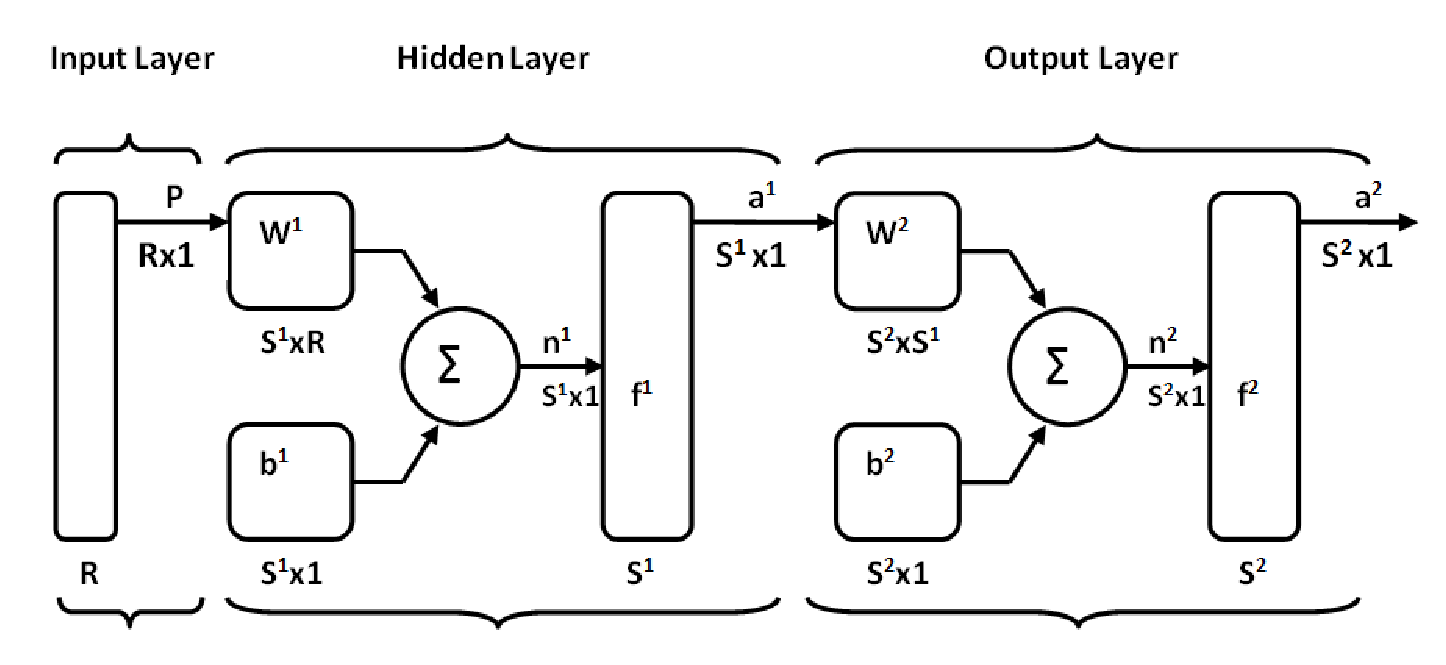
\includegraphics[width=350pt]{figures/ann/MLP.eps}
\caption{Feedforward Multilayer Perceptron.}
\label{figure_mlp}
\end{figure}


% $$ n^{k+1}(i)=\sum\limits_{i=1}^{Sk}w^{k+1}(i,j)a^{k}(j)+b^{k+1}(i). $$
\begin{equation}
n^{k+1}_i=\sum\limits_{i=1}^{Sk}w^{k+1}_{ij}a^{k}_{j}+b^{k+1}_i
\end{equation}\label{equation_feed_forward_input_to_k_layer}

where, $Sk$ is the number of neurons in the $k^{th}$ layer, $w^{k+1}_{ij}$ is the weight from $j^{th}$ neuron of layer $k$ to neuron $i$ of the layer $k+1$, $a^{k}_{j}$ is the output of neuron $j$ from the layer $k$ and $b^{k+1}_{i}$ is the bias connected to $i^{th}$ neuron in the layer $k+1$.

The output of unit $I$ will be,
%$$ a^{k+1}(i)=f^{k+1}(n^{k+1}(i))  $$
\begin{equation}
a^{k+1}_{i}=f^{k+1}(n^{k+1}_{i})
\end{equation}\label{equation_feed_forward_output_from_k_layer}

where, $f^{k+1}(\cdot)$ is the activation function (see appendix \ref{appendix_activation_functions}) used in layer $k+1$.

For a $M$ layer network the system equations in the matrix form are given by

\begin{align}\label{equation_feed_forward_step_in_matrix}
a^{0}&=p\\
a^{k+1}&= f^{k+1}(W^{k+1}a^k+b^{k+1}), k=0,1,2,...,M-1
\end{align}

where, $p$ is the input layer of the network.

The network learns association between a given set of input-output pairs ${(p_i,t_i), i=1,2,...,Q}$ for $Q$ number of training samples.


%The 

 index for the network is given as,
%$$ V=\dfrac{1}{2}\sum\limits_{q=1}^{Q}(t_q-a^M_q)=\dfrac{1}{2}\sum\limits_{q=1}^{Q}e^T_q e_q $$
%where $a^M_q$ is the output of the network when the $q^{th}$ input, $p_q$ is presented and $e_q=t_q-a^M_q$ is the error for the $q^{th}$ input.

Now, next step of calculating feed forward quantities for all layers in the network is the back propagation training. In this phase, we decide how neural network learn weights and biases with minimizing the generalization error. The quantity of weight and bias to adjust in the network parameters is send back to network from output layer to first hidden layer. In this research work, Levenberg-Marquardt Backpropagation Learning and Gradient Descent with Momentum \& Adaptive Learning Rate are applied for learning the network parameters. Levenberg-Marquardt Backpropagation Learning algorithm is described in the section \ref{section_lm_algorithm} and Gradient Descent with Momentum \& Adaptive Learning rate algorithm is described in the section \ref{section_gdma}.

\subsubsection{Levenberg-Marquardt Learning Algorithm}\label{section_lm_algorithm}

Many algorithms focus on standard numerical optimization, i.e, using alternative methods to heuristic based optimizations for computing the weights associated with network connections. The most popular algorithms for this optimization are the conjugate gradient and Newton’s methods. Newton’s method is considered to be more efficient in the speed of convergence, but its storage and  computational requirements go up as the square of the size of the network.
%  \cite{Hagan1994}. The LM algorithm is an approximation to Newton’s method [Moré77].
The LM algorithm is efficient in terms of high speed of convergence and reduced memory requirements compared to the two previous methods. In general, with networks that contain up to several hundred weights, the LM algorithm has the fastest convergence \cite{Hagan1994}.

For LM , the performance index to be minimized is defined as,
\begin{equation}\label{lm_performance_index}
F(w)=\sum\limits_{p=1}^{Q}{\sum\limits_{k=1}^{K}(t_{kp}-a_{kp})^2}
\end{equation}

where, $w=[w_1 $ $ w_2 $ $ w_3 $ $ ...$ $  w_N]^T$ consists of all the weights of the network (including bias), $t_{kp}$ is the target value of the $k^{th}$ output and $p^{th}$ input pattern, $a_{kp}$ is the actual value of the $k^{th}$ output and $p^{th}$ input pattern, $N$ is the number of weights, and $K$ is the number of the network outputs.

Equation (\ref{lm_performance_index}) can be written as,
\begin{equation}\label{equation_lm_error}
F(w)=E^TE
\end{equation}
where
$ E=[e_{11}$ $...$ $ e_{K1} $ $ e_{12}$ $...$ $ e_{K2}$ $ ...$ $ e_{1P} $ $...$ $ e_{KQ}]^T$, 

$ e_{kp}=t_{kp}-a_{kp}, $ $ k=1,2,...,K, $ $ p=1,2,...,Q$
where E is the cumulative error vector (for all input patterns).
From equation (\ref{equation_lm_error}) the Jacobian matrix is defined as,

\begin{equation}\label{jacobian_matrix}
 J=
\begin{bmatrix}
\frac{\partial{e_{11}}}{\partial{w_{1}}} & \frac{\partial{e_{11}}}{\partial{w_{2}}} & ... & \frac{\partial{e_{11}}}{\partial{w_{N}}} \\

\frac{\partial{e_{21}}}{\partial{w_{1}}} & \frac{\partial{e_{21}}}{\partial{w_{2}}} & ... & \frac{\partial{e_{21}}}{\partial{w_{N}}} \\

...&...&...&...&\\

\frac{\partial{e_{K1}}}{\partial{w_{1}}} & \frac{\partial{e_{K1}}}{\partial{w_{2}}} & ... & \frac{\partial{e_{K1}}}{\partial{w_{N}}} \\

...&...&...&...&\\

\frac{\partial{e_{1Q}}}{\partial{w_{1}}} & \frac{\partial{e_{1Q}}}{\partial{w_{2}}} & ... & \frac{\partial{e_{1Q}}}{\partial{w_{N}}} \\

\frac{\partial{e_{2Q}}}{\partial{w_{1}}} & \frac{\partial{e_{2Q}}}{\partial{w_{2}}} & ... & \frac{\partial{e_{2Q}}}{\partial{w_{N}}} \\
...&...&...&...&\\

\frac{\partial{e_{KQ}}}{\partial{w_{1}}} & \frac{\partial{e_{KQ}}}{\partial{w_{2}}} & ... & \frac{\partial{e_{KQ}}}{\partial{w_{N}}} \\
\end{bmatrix}
\end{equation}

The increment of weights $\Delta{w}$ at iteration $t$ can be obtained as follows:
\begin{equation}\label{equation_delta_w}
%\Delta{w}=(J^T_tJ_t+\mu_tI)^{-1}J^T_tE_t
\Delta{w}=-(J^TJ+\mu I)^{-1}J^TE
\end{equation}
where, $I$ is identity matrix, $\mu$ is a learning parameter and $J$ is Jacobian of $K$ output errors with respect to $N$ weights of the neural network.

Now, network weights are calculated using the following equation,
\begin{equation}\label{equation_new_weight}
w_{t+1}=w_t+\Delta{w}
\end{equation}


 For $\mu=0$, it becomes the Gauss-Newton method. For very large value of $\mu$ the \ac{lm} algorithm becomes the steepest decent algorithm. The learning parameter $\mu$  is automatically adjusted at each iteration to meet the convergence criteria. The \ac{lm} algorithm requires computation of the Jacobian matrix $J$ at each iteration and inverse of $J^TJ$ matrix of dimension $N$x$N$. This large dimensionality of \ac{lm} algorithm is sometimes unpleasant to large size neural network.

The learning parameter $\mu$ is updated in each iteration as follows. Whenever the $F(w)$ value is decreases, $\mu$ is multiplied by decay rate $\beta_{inc}$, whenever, $F(w)$ is increases, $\mu$ is divided by decay rate $\beta_{dec}$ in new step.

The \ac{lm} Back-propagation training is illustrated in the Algorithm \ref{algorithm_lm}.

\begin{algorithm}
\caption{Levenberg-Marquardt Back-propagation Algorithm}
\label{algorithm_lm}
\begin{algorithmic}[1]
\STATE Initialize the weights using Nguyen-Widrow weight initialization algorithm (see Appendix \ref{algorithm_appendix_nguyen_widrow_weight_initialization}) and parameter $\mu$.
\STATE Compute the sum of the squared errors over all inputs $F(w)$.
\STATE Solve Eq.(\ref{equation_delta_w}) to obtain the increment of weights.
\STATE Recompute the sum of squared errors $F(w)$ using $w+\Delta{w}$ as trial w, and adjust
\IF { trial $F(w)$ $\leq$ $F(w)$ in Step 2}
\STATE $w=w+\Delta{w}$
\STATE $\mu=\mu.\beta_{inc}$
\STATE Goto Step 2.
\ELSE
\STATE $\mu=\frac{\mu}{\beta_{dec}}$
\STATE  Goto Step 4.
\ENDIF
\end{algorithmic}
\end{algorithm}
\pagebreak
\subsubsection{Gradient descent with momentum and adaptive learning rate}
\label{section_gdma}
Gradient descent with momentum and variable learning rate is heuristic based optimization technique, developed from an analysis of the performance of the standard steepest descent algorithm, used for learning the feed-forward back-propagation neural network. It has a good convergence capacity than other heuristic based technique.


The term momentum controls feedback loop and help to overcome at the situation of noisy gradient, so that local minima can be passed without stoking. Momentum Adds a percentage of the last movement to the current movement. Momentum allows a network to respond not only to the local gradient, but also to recent trends in the error surface.

The term adaptive learning rate plays important role for fast convergence. The learning rate automatically changes while learning the patterns. For each iteration of learning, if the performance decreases toward the goal, then the learning rate is increased by the factor $\eta_{inc}$. If the performance increases by more than the factor $\eta_{max\_inc}$, the learning rate is adjusted by the factor $\eta_{dec}$ and the change that increased the performance is not made.

To learn the association between a given set of input-output pairs ${(p_i,t_i), i=1,2,...,Q}$ for $Q$ number of training samples, the performance index (given in Eq.\ref{lm_performance_index}) should be minimized.

The gradient of error function is the partial derivative of error function with respect to network weights and biases. It is given as,
\begin{equation}\label{equation_gradient_of_error}
\nabla{F}=\frac{\delta F }{\delta  w^k_{ij}}
\end{equation}

Change in weight for iteration $t+1$ is given by,
\begin{equation}\label{equation_gdma}
\Delta w(t+1)=\mu \Delta w(t) + (1-\mu)\eta \nabla{F}
\end{equation}
where, $\mu$ is the momentum constant and $\eta$ is the learning rate.

Now, Weight is adjusted by,
\begin{equation}\label{equation_gdma}
w(t+1)=w(t) + \Delta w(t+1)
\end{equation}

%The performance of the algorithm is very sensitive to the proper
%setting of the learning rate.If the learning rate is too small, the
%algorithm takes too long to converge. It is not practical to determine the
%optimal setting for the learning rate before training, and, in fact, the optimal
%learning rate changes during the training process, as the algorithm moves
%across the performance surface.

\newpage
\subsection{Radial Basis Function Network}
\label{section_radial_basis_function}

Radial-basis function network is used to perform a complex pattern classification task, the problem basically solved by transforming it into a high dimensional space in a non-linear manner. Non linear separability of complex patterns is justified by Cover's theorem,which stated as, ``A complex pattern-classification problem cast in a high dimensional space non-linearly is more likely to be linearly separable than in a low-dimensional space''.

Radial basis functions are embedded into a two layer feed-forward network. Such a  network is characterized by a set of inputs and set of outputs. In between the inputs and outputs, there is a layer of processing units called hidden units. Each of them implements a radial basis function. Generally, there is a single hidden layer. In pattern classification problem, inputs represent feature values, while each output corresponds to a class. A general \ac{rbf} Neural Network Architecture is given in Figure \ref{figure_rbf}.

\begin{figure}[h]
\centering
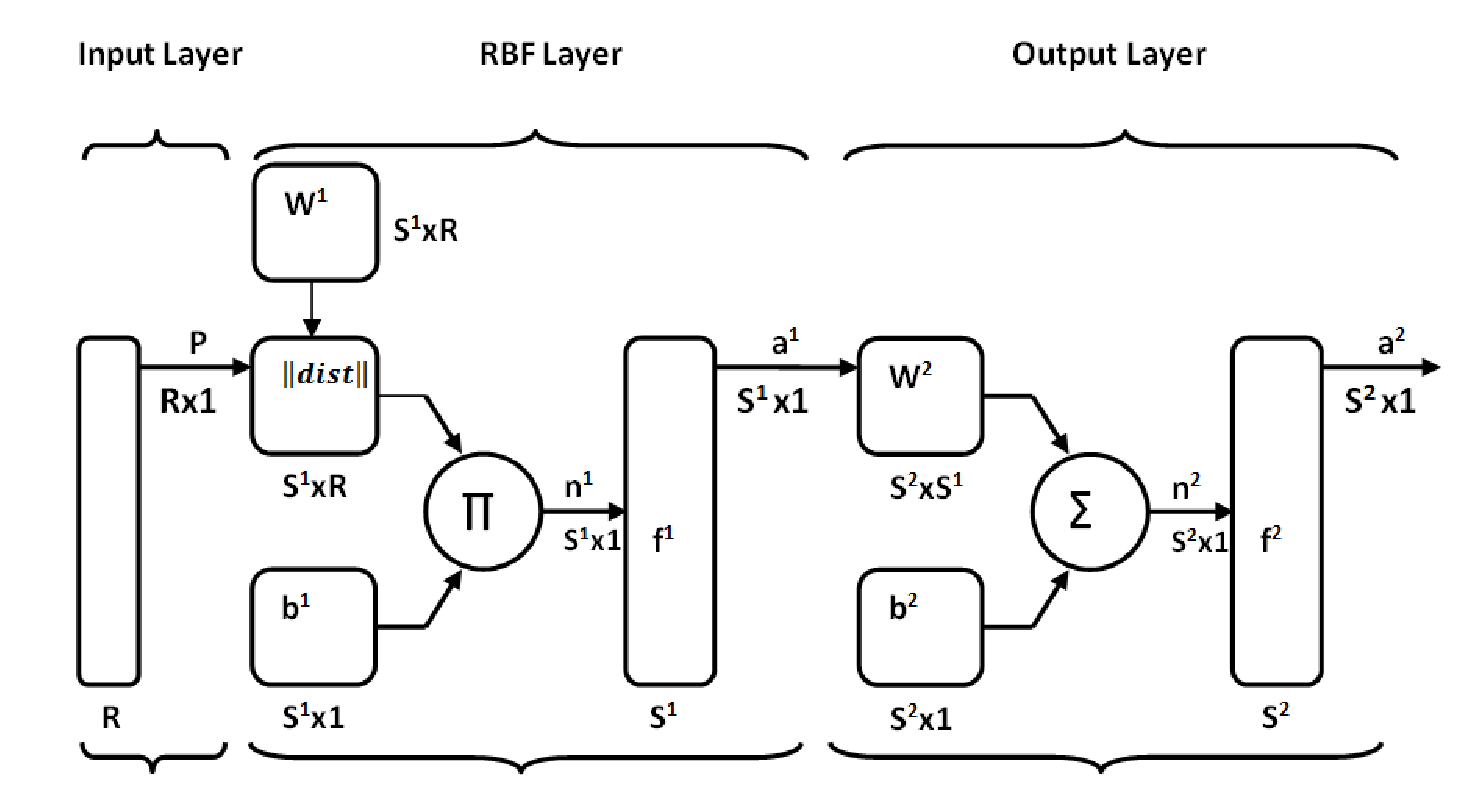
\includegraphics[width=350pt,height=170pt]{figures/ann/RBF.eps}
\caption{RBF Neural Network.}
\label{figure_rbf}
\end{figure}
Let the input vector $x=[x_1,x_2,...,x_R]^T$ is feed to RBF Network. The network output can be obtained by,

\begin{equation}\label{equation_rbf_network_output}
%t_k=\sum\limits_{j=1}^{M}w_{kj}\phi_j(\lVert x-c_j\rVert)+b_k
t_k=\sum\limits_{j=1}^{M}w_{kj}\phi_j(x)+b_k
\end{equation}
where $\phi_j(\cdot)$ denotes the radial basis function of the $j^{th}$ hidden neuron, $w_{kj}$ denotes the hidden-to-output weight from $j^{th}$ hidden neuron to $k^{th}$ output neuron, $b_k$ denotes the bias connected to $k^{th}$ output neuron, and $M$ denotes the total hidden neurons.

A radial basis function is a multidimensional function that describes the distance between a given input vector and a pre-defined centre vector. There are different types of radial basis function.  A normalized Gaussian function usually used as a radial basis function, which is given as,

\begin{equation}\label{equation_radial_basis_fuction}
\phi_j(x)=\exp(-\frac{\Vert x-\mu_j\Vert^2}{2\sigma^2_j})
\end{equation}
where, $\mu_j$ and $\sigma_j$ denote the centre and spread width of the $j^{th}$ neuron, respectively.

Generally, the \ac{rbfnn} training can be divided into two stages:
\begin{enumerate}
\itemsep0em
\item Determine the parameters of radial basis functions, i.e., Gaussian centre and spread width.
\item Determine the output weight $w$ with supervised learning method. Usually \ac{lms}.
\end{enumerate}
The first stage is very crucial, since the number location of centres in the hidden layer will influence the performance of the \ac{rbf} neural network directly. In the next section, the principle and procedure of self-structure \ac{rbf} algorithm will be described.

\subsubsection{Orthogonal Least Square Training Algorithm}\label{section_ols}

Orthogonal Least Squares is the most widely used supervised algorithm for radial basis neural network training. \ac{ols} is a forward stepwise regression procedure. Starting from a large pool of candidate centres, i.e., from training examples, \ac{ols} sequentially selects the centre that results in the largest reduction of sum-square-error at the output.

For $M$ basis vectors $\Phi=(\phi_1,\phi_2,...,\phi_M)$, orthogonal set $Q=(q_1,q_2,...,q_M)$ can be derived with the help of Grahm-Schmidt orthogonalization procedure as follows:

\begin{align}
q_1&=\phi_1 \label{q1} \\
\alpha_{ik}&=\frac{q^T_i\phi_k}{q^T_iq_i} \; 1\le i \le k \label{alpha_ik}\\
q_k&=\phi_k-\sum\limits_{i=1}^{k-1}\alpha_{ik}q_i \label{qk}\\
& for \; k=2,3,...,M \nonumber
\end{align}

The orthogonal set of basis vectors Q is linearly related to the original set $\Phi$ by the relationship $ \Phi=QA \label{orthogonal_representation}$ \cite{Chen1991}, where A is upper triangular matrix given by,

\begin{equation}
A=
\begin{bmatrix}
1&\alpha_{12}&...&\alpha_{1M}\\
0&1&&...\\
...&&&\alpha_{M-1,M}\\
0&...&0&1
\end{bmatrix}
\end{equation}

Using this orthogonal representation, the \ac{rbf} solution is expressed as,
\begin{equation}
T=\Phi W= QG
\end{equation}
and the \ac{ls} solution for the weight vector $G$ in the orthogonal space is,

\begin{equation}
G=(Q^TQ)^{-1}Q^TT
\end{equation}

Since Q is orthogonal, $Q^TQ$ is then diagonal and each component of G can be extracted independently without ever having to compute a pseudo-inverse matrix as,

\begin{equation}\label{ols_pseudo_inverse}
g_i=\frac{q^T_iT}{q^T_iq_i}
\end{equation}

The sum of squares of the target vector T is given as,

\begin{equation}
T^TT=\sum\limits_{i=1}^{M}g^2_iq^T_iq_i+E^TE
\end{equation}

\ac{ols} select a subset of regressors in stepwise forward manner by selecting the regressor $q_i$,which contributes to reduction of the error (relative to the total $T^TT$) by,
\begin{equation}\label{ols_error}
[err]_i=\frac{g^2_iq^T_iq_i}{T^TT}
\end{equation}

The summary of Orthogonal Least Square \ac{rbf} training \cite{Chen1991} is given in Algorithm \ref{algorithm_ols}.

\begin{algorithm}
\caption{OLS Algorithm}
\label{algorithm_ols}
\begin{algorithmic}[1]
\STATE At the first step,for $1\le i\le M$, compute
\STATE \qquad\qquad Orthogonalize vector: $q^{(i)}_1=\phi_i$
\STATE \qquad\qquad Compute \ac{ls} Solution:	$g^{(i)}_1=\frac{q^{{(i)}^T}_1T}{q^{{(i)}^T}_1q^{(i)}_1}$
\STATE \qquad\qquad Compute error reduction: $[err]^{(1)}_i=\frac{g^{{(i)}^2}_1q^{{(i)}^T}_1q^{(i)}_1}{T^TT}$
\STATE \quad select regressor that yields highest reduction in error $q_1=\arg_{q^{(i)}_1}\max[err]^{(i)}_1=\phi_{i_1}$


\STATE At the $k^{th}$ step, for $1\le i\le M$, and $i$ not already selected
\STATE \qquad\qquad Orthogonalize vector: $\alpha^{(i)}_{jk}=\frac{q^T_j\phi_i}{q^T_jq_j} \;, q^{(i)}_k=\phi_i-\sum\limits_{i=1}^{k-1}\alpha^{(i)}_{jk}q_j \;, for 1\le j \le k $
\STATE \qquad\qquad Compute \ac{ls} Solution:	$g^{(i)}_k=\frac{q^{{(i)}^T}_kT}{q^{{(i)}^T}_kq^{(i)}_k}$
\STATE \qquad\qquad Compute error reduction: $[err]^{(i)}_k=\frac{g^{{(i)}^2}_kq^{{(i)}^T}_kq^{(i)}_k}{T^TT}$
\STATE \quad select regressor $q_k=\arg_{q^{(i)}_k}\max[err]^{(i)}_k=\phi_{i_k}-\sum\limits_{j=1}^{k-1}\alpha_{jk}q_j$

\STATE Stop at iteration M if residual error falls below pre-specified threshold $\epsilon$
\STATE \qquad\qquad\qquad $1- \sum\limits_{j=1}^{M}[err]_j \le \epsilon $
\STATE The regressors $\lbrace{\phi_{i_1},\phi_{i_2},\cdots,\phi_{i_M}}\rbrace$ define the final subset of RBF centers.
\end{algorithmic}
\end{algorithm}

\subsection{Performance Metrics}
Performance of the recognition systems is evaluated on the basis of the metrics described below:
\begin{enumerate}
\itemsep0em
\item \textbf{Recognition Rate:} Number of instances that were classified correctly out of the total instances.
\item \textbf{Misclassification Rate:} Number of instances that were classified incorrectly out of the total instances.
\item \textbf{Model Build Time:} Time taken to train a classifier on a given data set.
\end{enumerate}

